\documentclass[
11pt % The default document font size, options: 10pt, 11pt, 12pt
%codirector, % Uncomment to add a codirector to the title page
]{charter} 


% El títulos de la memoria, se usa en la carátula y se puede usar el cualquier lugar del documento con el comando \ttitle
\titulo{Implementación de técnicas de visión artificial para la identificación de frutos de duraznero} 

% Nombre del posgrado, se usa en la carátula y se puede usar el cualquier lugar del documento con el comando \degreename
%\posgrado{Carrera de Especialización en Inteligencia Artificial} 
%\posgrado{Carrera de Especialización en Internet de las Cosas} 
\posgrado{Carrera de Especialización en Inteligencia Artificial}
%\posgrado{Maestría en Sistemas Embebidos} 
%\posgrado{Maestría en Internet de las cosas}
% IMPORTANTE: no omitir titulaciones ni tildación en los nombres, también se recomienda escribir los nombres completos (tal cual los tienen en su documento)
% Tu nombre, se puede usar el cualquier lugar del documento con el comando \authorname
\autor{Ing. Sergio Hinojosa}

% El nombre del director y co-director, se puede usar el cualquier lugar del documento con el comando \supname y \cosupname y \pertesupname y \pertecosupname
\director{Ing. Maxim Dorogov}
\pertenenciaDirector{FIUBA} 
\codirector{} % para que aparezca en la portada se debe descomentar la opción codirector en los parámetros de documentclass
\pertenenciaCoDirector{}

% Nombre del cliente, quien va a aprobar los resultados del proyecto, se puede usar con el comando \clientename y \empclientename
\cliente{Dr. Gerardo Sánchez}
\empresaCliente{INTA}
 
\fechaINICIO{18 de junio de 2024}		%Fecha de inicio de la cursada de GdP \fechaInicioName
\fechaFINALPlan{13 de agosto de 2024} 	%Fecha de final de cursada de GdP
\fechaFINALTrabajo{- de - de 2024}	%Fecha de defensa pública del trabajo final


\begin{document}

\maketitle
\thispagestyle{empty}
\pagebreak


\thispagestyle{empty}
{\setlength{\parskip}{0pt}
\tableofcontents{}
}
\pagebreak


\section*{Registros de cambios}
\label{sec:registro}


\begin{table}[ht]
\label{tab:registro}
\centering
\begin{tabularx}{\linewidth}{@{}|c|X|c|@{}}
\hline
\rowcolor[HTML]{C0C0C0} 
Revisión & \multicolumn{1}{c|}{\cellcolor[HTML]{C0C0C0}Detalles de los cambios realizados} & Fecha      \\ \hline
0      & Creación del documento &\fechaInicioName \\ \hline
1      & Se completa hasta el punto 5 inclusive & {2} de {Julio} de 2024 \\ \hline
2      & Se completa hasta el punto 9 inclusive & {9} de {Julio} de 2024 \\ \hline
3      & Se completa hasta el punto 12 inclusive  & {22} de {Julio} de 2024 \\ \hline
4      & Se completa el plan  & {31} de {Julio} de 2024 \\ \hline
4.1    & Se completa el plan  & {4} de {Agosto} de 2024 \\ \hline
% Si hay más correcciones pasada la versión 4 también se deben especificar acá

\end{tabularx}
\end{table}

\pagebreak



\section*{Acta de constitución del proyecto}
\label{sec:acta}

\begin{flushright}
Buenos Aires, \fechaInicioName
\end{flushright}

\vspace{2cm}

Por medio de la presente se acuerda con \authorname\hspace{1px} que su Trabajo Final de la \degreename\hspace{1px} se titulará ``\ttitle'' y consistirá en la implementación de un algoritmo que permita identificar y cuantificar frutos de duraznos a partir de imágenes de árboles tomadas a campo. El trabajo tendrá un presupuesto preliminar estimado de 600 horas y un costo estimado de US\$18267, con fecha de inicio el \fechaInicioName\hspace{1px} y fecha de presentación pública en el mes de diciembre de 2024.%\fechaFinalName.

Se adjunta a esta acta la planificación inicial.

\vfill

% Esta parte se construye sola con la información que hayan cargado en el preámbulo del documento y no debe modificarla
\begin{table}[ht]
\centering
\begin{tabular}{ccc}
\begin{tabular}[c]{@{}c@{}}Dr. Ing. Ariel Lutenberg \\ Director posgrado FIUBA\end{tabular} & \hspace{2cm} & \begin{tabular}[c]{@{}c@{}}\clientename \\ \empclientename \end{tabular} \vspace{2.5cm} \\ 
\multicolumn{3}{c}{\begin{tabular}[c]{@{}c@{}} \supname \\ Director del Trabajo Final\end{tabular}} \vspace{2.5cm} \\
\end{tabular}
\end{table}



\newpage
\section{1. Descripción técnica-conceptual del proyecto a realizar}
\label{sec:descripcion}
\subsection{Contexto de la implementación}

Contar de forma manual la cantidad frutos que posee un árbol en una plantación agrícola resulta una tarea laboriosa, lenta y propensa a errores. No obstante, conocer estos datos tiene diversas aplicaciones importantes que, debido a su dificultad, no están siendo abordadas. Para un productor, por ejemplo, saber la cantidad de frutos que posee una muestra de su lote durante el raleo\footnote{Descarte de una parte de los frutos para que los restantes tomen más nutrientes de la planta y puedan alcanzar tamaño comercial} le permite calcular la intensidad a aplicar. Además, al momento de la cosecha, le permite tener una estimación de su producción.

\subsection{Objetivo del proyecto}

Este proyecto busca proporcionar al productor:
\begin{itemize}
	\item Precisión y eficiencia: conteo de manera precisa y rápida.
	\item Ahorro de tiempo y costos: reducción del tiempo y de costos asociados con la mano de obra requerida para esta tarea.
	\item Optimización del rendimiento agrícola: permitir toma de decisiones informadas sobre la gestión del cultivo, la cosecha y la planificación de la mano de obra.
	\item Monitoreo temprano de la producción.
\end{itemize}

Por otro lado, los algoritmos a desarrollar resultan una herramienta muy útil, ya que permiten la obtención de un gran volumen de datos que pueden vincularse con diferentes características de interés, tales como:

\begin{itemize}
	\item Porcentaje de cuajado: relacionado con la producción.
	\item Potencial de raleo: capacidad de genotipo a soportar mayor o menor raleo.
	\item Rendimiento.
\end{itemize}

A esto se lo denomina fenotipo y esta herramienta fenómica será fundamental para
alimentar modelos de IA que combinan datos genómicos con variables ambientales.

El siguiente diagrama de bloques ilustra el pipeline del sistema, los diferentes subsistemas involucrados y el flujo de datos:

\begin{figure}[htpb]
\centering 
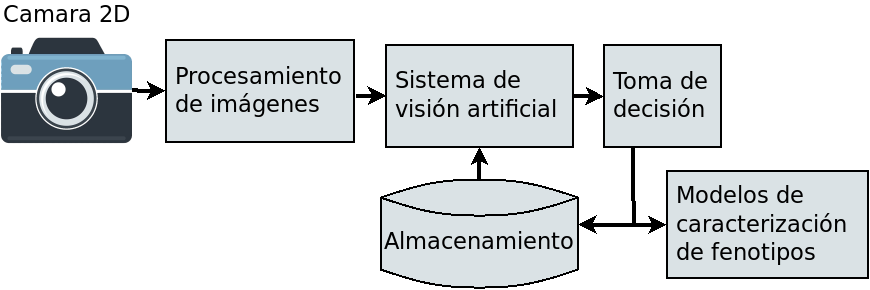
\includegraphics[width=.85\textwidth]{./Figuras/diagrama.png}
\caption{Diagrama en bloques del sistema.}
\label{fig:diagBloques}
\end{figure}

\vspace{25px}



\section{2. Identificación y análisis de los interesados}
\label{sec:interesados}

\begin{table}[ht]
%\caption{Identificación de los interesados}
%\label{tab:interesados}
\begin{tabularx}{\linewidth}{@{}|l|X|X|l|@{}}
\hline
\rowcolor[HTML]{C0C0C0} 
Rol           & Nombre y Apellido & Organización 	& Puesto 	\\ \hline
%Auspiciante   &                   &              	&        	\\ \hline
Cliente       & \clientename      &\empclientename	& Director Científico Biotango Technologies SAS\\ \hline
%Impulsor      &                   &              	&        	\\ \hline
Responsable   & \authorname       & FIUBA        	& Alumno 	\\ \hline
%Colaboradores &                   &              	&        	\\ \hline
Orientador    & \supname	      & \pertesupname 	& Director del Trabajo Final \\ \hline
%Equipo        & miembro1 \newline 
%				miembro2          &              	&        	\\ \hline
%Opositores    &                   &              	&        	\\ \hline
%Usuario final &                   &              	&        	\\ \hline

\end{tabularx}
\end{table}

Cliente: el Dr. Gerardo Sanchez tiene más de 20 años de experiencia en biotecnología frutícola, colaborará en los requerimientos y en la válidación de los modelos desarrollados.

Orientador: el Ing. Maxim Dorogov posee gran experiencia y conocimientos en el área de visión artificial. Es orientador desde los aspectos técnicos y participa en definir los objetivos del proyecto.

\section{3. Propósito del proyecto}
\label{sec:proposito}

El propósito de este proyecto es desarrollar un sistema informático capaz de detectar y contar los frutos de un duraznero en el árbol a partir de imágenes tomadas por una cámara 2D.

\section{4. Alcance del proyecto}
\label{sec:alcance}


El proyecto incluye:
\begin{itemize}
	\item Procesamiento de la imagen tomada por un celular.
	\item Detección del árbol a analizar.
	\item Conteo de los frutos.
\end{itemize}

El proyecto no incluye:
\begin{itemize}
	\item Procesamiento de imágenes en blanco y negro.
	\item Procesamiento de video.
	\item Implementación industrial. No se realizará un deploy en ningún sistema embebido ni en la nube, el sistema se mantendrá en un entorno de desarrollo.
\end{itemize}


\section{5. Supuestos del proyecto}
\label{sec:supuestos}

Para el desarrollo del presente proyecto se supone que se contará con:

\begin{itemize}
    \item Horas de trabajo del desarrollador y del director del proyecto.
	\item Un ordenador con placa gráfica dedicada.
	\item Banco de imágenes de campo reales para el entrenamiento del sistema.
	\item No será necesario una inversión en hardware.
	\item No se espera una precisión del 100 \%. Se definirá un margen aceptable.
\end{itemize}

\section{6. Requerimientos}
\label{sec:requerimientos}

\begin{enumerate}
	\item Requerimientos funcionales:
	\begin{enumerate}
		\item El sistema debe ser capaz de identificar y cuantificar frutos tanto en estado inmaduro o maduro a partir de fotos de árboles tomadas en la plantación. 
		\item El sistema debe ser capaz de analizar fotos en formato .jpeg.
		\item El sistema deberá indicar el grado de confianza de la detección y el error esperado en las mediciones.
		\item El sistema debe mostrar los resultados en una interfaz gráfica y debe exportar los resultados a formato .cvs 
		\item Los dataset y código en repositorios deben mantenerse NO abiertos, de modo de mantener la confidencialidad del trabajo.
		\item El usuario debe poder analizar una foto individual o un grupo de fotos, por lo menos grupos de 20 imágenes.
		\item El usuario debe ser capaz de cambiar el nivel de confianza para modificar la detección.
	\end{enumerate}

	\item Requerimientos de documentación:
	\begin{enumerate}
		\item Se debe proveer el códigos base.
		\item Se deben describir los ensayos y condiciones para la reporducción de los mismos.
		\item Se debe generar el informe de avance y la memoria final del trabajo.
		\item Se debe proveer un manual de instrucciones para la instalación y uso.
	\end{enumerate}
	
	\item Requerimientos de testing:
	\begin{enumerate}
		\item El modelo debe ser entrenado a partir de modelos pre-entrenados utilizando la técnica de \textit{transfer learning}.
		\item El entrenamiento del modelo debe realizarse a partir de un dataset creado con imágenes propias y de terceros respetando los derechos de uso establecidos por los mismos.
		\item El entrenamiento y las pruebas en los datasets de validación y testing deben ser llevadas adelante en notebooks escritas en lenguaje de programación Python 3.8 o superior.
	\end{enumerate}
	
	\item Requerimientos de la interfaz:
	\begin{enumerate}
		\item La intefaz debe ser intuitiva, con capacidad de cargar las fotos de manera sencilla.
	\end{enumerate}

\end{enumerate}

\section{7. Historias de usuarios (\textit{Product backlog})}
\label{sec:backlog}

El criterio establecido para la asignación de los puntajes de las historias de usuario se basa en los criterios:
\begin{enumerate}
	\item Esfuerzo requerido en tiempo.
	\item Complejidad de la tarea.
	\item Riesgo asociado.
\end{enumerate}
Cada uno de los criterios individuales puede tener un valor entre 0 (bajo) y 5 (alto). El puntaje final será la suma de los puntajes individuales y se le asignará el valor más próximo de los valores de la serie de Fibonacci: 1, 2, 3, 5, 8, 13, 20.

\begin{itemize}
\item Como usuario, quiero un sistema de visión artificial que detecte y cuente automáticamente la cantidad de duraznos en mis árboles, para poder monitorear y gestionar mejor mi producción.
	\begin{itemize}
	\item Complejidad: 4
	\item Dificultad: 3
	\item Incertidumbre: 3
	\item \textit{Story points}: 13 
	\end{itemize}
\end{itemize}

\begin{itemize}
\item Como usuario, quiero poder capturar imágenes de mis árboles utilizando una cámara y poder subirla al sistema para el conteo de los frutos.
	\begin{itemize}
	\item Complejidad: 1
	\item Dificultad: 1
	\item Incertidumbre: 2
	\item \textit{Story points}: 5 
	\end{itemize}
\end{itemize}

\begin{itemize}
\item Como usuario, quiero poder configurar parámetros del sistema (como la sensibilidad de detección), para ajustar la precisión del conteo según las condiciones específicas de mi plantación.
	\begin{itemize}
	\item Complejidad: 4
	\item Dificultad: 2
	\item Incertidumbre: 4
	\item \textit{Story points}: 8 
	\end{itemize}
\end{itemize}

\begin{itemize}
\item Como usuario, quiero recibir un reporte con la cantidad de duraznos detectados en cada árbol, para poder tomar decisiones informadas sobre mi cultivo.
	\begin{itemize}
	\item Complejidad: 2
	\item Dificultad: 2
	\item Incertidumbre: 2
	\item \textit{Story points}: 8 
	\end{itemize}
\end{itemize}

\begin{itemize}
\item Como desarrollador, quiero establecer un entorno de desarrollo escalable, bien documentado y organizado para facilitar la mejora continua del sistema.
	\begin{itemize}
	\item Complejidad: 3
	\item Dificultad: 5
	\item Incertidumbre: 3
	\item \textit{Story points}: 13 
	\end{itemize}
\end{itemize}

\begin{itemize}
\item Como desarrollador, quiero crear un sistema de notificaciones de error y logueo que alerte sobre los problemas en la detección y sea más sencillo remediar bugs o corregir parámetros de configuración.
	\begin{itemize}
	\item Complejidad: 3
	\item Dificultad: 3
	\item Incertidumbre: 2
	\item \textit{Story points}: 8 
	\end{itemize}
\end{itemize}

\begin{itemize}
\item Como desarrollador, quiero diseñar una base de datos para almacenar las imágenes y los resultados de detección, para poder acceder y analizar los datos históricos.
	\begin{itemize}
	\item Complejidad: 2
	\item Dificultad: 2
	\item Incertidumbre: 2
	\item \textit{Story points}: 8 
	\end{itemize}
\end{itemize}

\section{8. Entregables principales del proyecto}
\label{sec:entregables}

Los entregables del proyecto son:

\begin{itemize}
	\item Documento de arquitecutra de software.
	\item Notebooks desarrolladas para el entrenamiento del modelo.
	\item Datasets utilizados.
	\item Manual de usuario.
	\item Informe de avance.
	\item Informe final.
\end{itemize}

\section{9. Desglose del trabajo en tareas}
\label{sec:wbs}

\begin{enumerate}
\item Gestión del proyecto (50 h)
	\begin{enumerate}
	\item Estudio de necesidades. (6 h)
	\item Análisis de requerimientos. (6 h)
	\item Análisis de factibilidad. (6 h)
	\item Entregables GdP hasta sección 5. (4 h)
	\item Entregables GdP hasta sección 9. (4 h)
	\item Entregables GdP hasta sección 12. (6 h)
	\item Entregables GdP hasta sección 15. (6 h)
	\item Elaboración presentación GdP. (6 h)
	\item Revisión y correcciones entregables GdP. (6 h)
	\end{enumerate}
	
\item Investigación preliminar (110 h)
	\begin{enumerate}
	\item Investigación de modelos de detección y clasificación de objetos. (40 h)
	\item Desarrollo de tests de performance para la aplicación. (40 h)
	\item Análisis de los resultados y selección del modelo final. (30 h)
	\end{enumerate}
	
\item Recopilación de imágenes para los datasets (90 h)
	\begin{enumerate}
	\item Búsqueda de datasets de terceros. (20 h)
	\item Captura de imágenes. (30 h)
	\item Preparación del dataset. (25 h)
	\item Refinamiento y seleccción final. (15 h)
	\end{enumerate}

\item Entrenamiento de la red neuronal (130 h)
	\begin{enumerate}
	\item Desarrollo del modelo. (50 h)
	\item Entrenamiento del modelo. (40 h)
	\item Ajuste de hiperparámetros. (30 h)
	\item Refinamiento del dataset. (10 h)
	\end{enumerate}
	
\item Desarrollo del sistema global (120 h)
	\begin{enumerate}
	\item Desarrollo de una interfaz de comandos de alto nivel. (40 h)
	\item Desarrollo del sistema de registro en base de datos. (20 h)
	\item Evaluación de desempeño del sistema. (20 h)
	\item Desarrollo de demos. (40 h)
	\end{enumerate}
	
\item Generación de entregables y proceso de cierre (100 h)
	\begin{enumerate}
	\item Inicio elaboración memoria técnica - Taller de Trabajo Final A. (40 h)
	\item Revisión y correcciones de la memoria. (5 h)
	\item Fin de elaboración memoria técnica - Taller de Trabajo Final B. (40 h)
	\item Revisión y correcciones de la memoria. (5 h)
	\item Elaboración presentación final. (8 h)
	\item Revisión y correcciones de la presentación final. (2 h)
	\end{enumerate}
\end{enumerate}

Cantidad total de horas: 600 horas.

\section{10. Diagrama de Activity On Node}
\label{sec:AoN}

En la figura 2, se muestra el diagrama Activity on Node del proyecto. Los tiempos de las tareas están expresados en horas.

Si bien se observa alguna paralelización de tareas, estas se realizarán de forma secuencial o intercalada debido a que solo habrá una persona trabajando en ellas.

En el diagrama se indica con un mayor grosor de flecha el camino crítico.

\begin{figure}[htpb]
\centering 
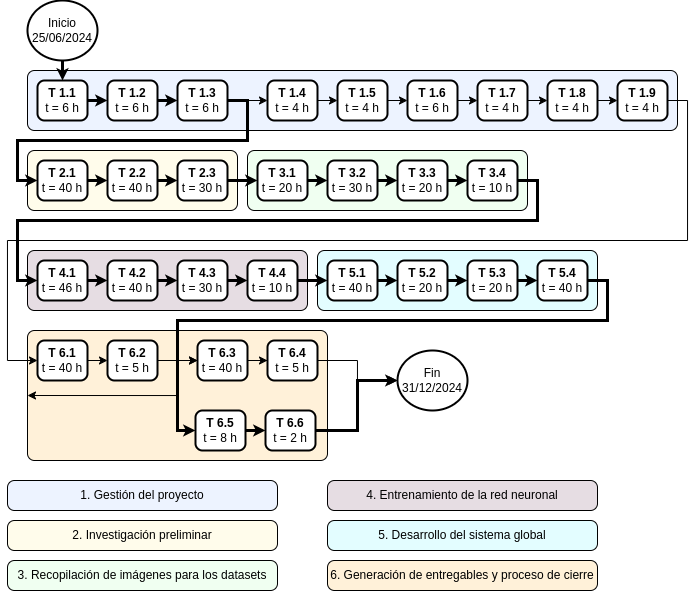
\includegraphics[width=.8\textwidth]{./Figuras/AoN.png}
\caption{Diagrama de \textit{Activity on Node}.}
\label{fig:AoN}
\end{figure}

Duración del camino crítico: 484 h.

\section{11. Diagrama de Gantt}
\label{sec:gantt}

\begin{landscape}
\begin{figure}[htpb]
\centering 
\includegraphics[height=.85\textheight]{./Figuras/Gantt.png}
\caption{Diagrama de Gantt.} %Modificar este título acorde.
\label{fig:diagGantt}
\end{figure}

\end{landscape}


\section{12. Presupuesto detallado del proyecto}
\label{sec:presupuesto}

A continuación se presenta el presupuesto detallado del proyecto expresado en dólares
estadounidenses:

\begin{table}[htpb]
\centering
\begin{tabularx}{\linewidth}{@{}|X|c|r|r|@{}}
\hline
\rowcolor[HTML]{C0C0C0} 
\multicolumn{4}{|c|}{\cellcolor[HTML]{C0C0C0}COSTOS DIRECTOS} \\ \hline
\rowcolor[HTML]{C0C0C0} 
Descripción &
  \multicolumn{1}{c|}{\cellcolor[HTML]{C0C0C0}Cantidad} &
  \multicolumn{1}{c|}{\cellcolor[HTML]{C0C0C0}Valor unitario} &
  \multicolumn{1}{c|}{\cellcolor[HTML]{C0C0C0}Valor total} \\ \hline
Horas de ingeniería & 
  \multicolumn{1}{c|}{580} &
  \multicolumn{1}{c|}{30} &
  \multicolumn{1}{c|}{17400} \\ \hline
Cómputo - Google cloud &
  \multicolumn{1}{c|}{6} &
  \multicolumn{1}{c|}{45} &
  \multicolumn{1}{c|}{270} \\ \hline
\multicolumn{3}{|c|}{SUBTOTAL} &
  \multicolumn{1}{c|}{17670} \\ \hline
\rowcolor[HTML]{C0C0C0} 
\multicolumn{4}{|c|}{\cellcolor[HTML]{C0C0C0}COSTOS INDIRECTOS} \\ \hline
\rowcolor[HTML]{C0C0C0} 
Descripción &
  \multicolumn{1}{c|}{\cellcolor[HTML]{C0C0C0}Cantidad} &
  \multicolumn{1}{c|}{\cellcolor[HTML]{C0C0C0}Valor unitario} &
  \multicolumn{1}{c|}{\cellcolor[HTML]{C0C0C0}Valor total} \\ \hline
\multicolumn{1}{|l|}{Viáticos} &
8   &
12   &
96   \\ \hline
\multicolumn{1}{|l|}{30 \% del costo directo} &
-   &
-   &
501   \\ \hline
\multicolumn{3}{|c|}{SUBTOTAL} &
  \multicolumn{1}{c|}{597} \\ \hline
\rowcolor[HTML]{C0C0C0}
\multicolumn{3}{|c|}{TOTAL} &
18267   \\ \hline
\end{tabularx}%
\end{table}

Al día de la fecha, 28 de Julio de 2024, el costo total es de \$17353650 (pesos argentinos).

\section{13. Gestión de riesgos}
\label{sec:riesgos}

En la identificación de los riesgos se utiliza una escala de 1 a 10 para cuantificar la probabilidad de ocurrencia y severidad. Se considera 1 como la mínima probabilidad y 10 la máxima.

Riesgo 1: registro de imágenes insuficientes para el entrenamiento del modelo.
\begin{itemize}
	\item Severidad (S): 9. El rendimiento del modelo entrenado depende directamente de la calidad del dataset recopilado.
	\item Probabilidad de ocurrencia (O): 6. La recopilación de imágenes en campo puede ser dificultosa y de baja calidad.
\end{itemize}

Riesgo 2: pobre resolución de las imágenes.
\begin{itemize}
	\item Severidad (S): 8. No solo es necesario una cantidad significativa de imágenes si no que también es importante la calidad de las mismas. Los modelos no se desempeñarían correctamente ocasionando un mal funcionamiento global del sistema.
	\item Probabilidad de ocurrencia (S): 3. La cámara sería seleccionada teniendo en cuenta los requerimientos y un margen de seguridad adecuado que cubra acualquier eventual
disminución de resolución causada por el encargado de tomar las imágenes y el preprocesamiento de las mismas.
\end{itemize}

Riesgo 3: mala precisión de los modelos entrenados.
\begin{itemize}
	\item Severidad (S): 8. Los malos resultados del modelo en la etapa de prueba pueden requerir mayores tiempos de entrenamiento e impactar en la viabilidad técnica del proyecto.
	\item Probabilidad de ocurrencia (O): 4. Los tiempos de entrenamiento son muy extensos y
muchas veces son una variable de ajuste necesaria.
\end{itemize}

Riesgo 4: no contar con suficiente capacidad de cómputo.
\begin{itemize}
	\item Severidad (S): 8. Trabajar con procesamiento de imágenes implica gran consumo de recursos de hardware. No contar con la capacidad de cómputo adecuada implicaría que las tareas se hagan más largas de lo estimado o que se requiera contratar servicios de cómputo más costoso.
	\item Probabilidad de ocurrencia (O): 3. El responsable posee un equipo adecuado y se contrata un servicio de cómputo en la nube que en principio es suficiente para el desarrollo.
\end{itemize}

Riesgo 5: falta de tiempo y/o recursos humanos para el desarrollo.
\begin{itemize}
	\item Severidad (S): 7. Se atrasarían las tareas, no se cumpliría con la planificación y quizás no se lograría completar el proyecto para la fecha de presentación establecida.
	\item Probabilidad de ocurrencia (O): 4. El proceso de etiquetado del dataset suele ser muy extenso y tedioso por lo que la estimación de tiempo para esa etapa podría ser errónea. La elección del modelo y el ajuste de hiperparámetros es también una tarea que podría variar a lo estimado por la complejidad de su desarrollo.
\end{itemize}

b) Tabla de gestión de riesgos: (El RPN se calcula como RPN=SxO)

\begin{table}[htpb]
\centering
\begin{tabularx}{\linewidth}{@{}|X|c|c|c|c|c|c|@{}}
\hline
\rowcolor[HTML]{C0C0C0} 
Riesgo & S & O & RPN & S* & O* & RPN* \\ \hline
Registro de imágenes insuficientes para el entrenamiento del modelo & 9 & 6 & 54 & 5 & 6 & 30 \\ \hline
Pobre resolución de las imágenes & 8 & 3 & 24 & - & - & - \\ \hline
Mala precisión de los modelos entrenados & 8 & 4 & 32 & 6 & 3 & 18 \\ \hline
No contar con suficiente capacidad de cómputo & 8 & 3 & 24 & - & - & - \\ \hline
Falta de tiempo y/o recursos humanos para el desarrollo & 7 & 5 & 35 & 7 & 4 & 28 \\ \hline
\end{tabularx}%
\end{table}

Criterio adoptado: se tomarán medidas de mitigación en los riesgos cuyos números de RPN sean mayores a 30.


Plan de mitigación de los riesgos que originalmente excedían el RPN máximo establecido:

\textbf{Riesgo 1 - Datos insuficientes}. Plan de mitigación: lograr el mayor avance posible con datos suplementarios. Existen fuentes de datos públicos que se pueden adaptar a esta problemática, el durazno es una fruta muy común.
\begin{itemize}
	\item Severidad (S): 5. Es posible favorecer el rendimiento de los modelos con técnicas como \textit{transfer learning} o \textit{one-shot learning} con la variabilidad de datos proporcionado con datasets públicos, aunque no sean específicamente de lo especificado en la problemática a solucionar. De todos modos no es el escenario más favorable.
	\item Probabilidad de ocurrencia (O): 6. La probabilidad de ocurrencia no se modifica.
\end{itemize}
Nueva asignación de S y O: 30.

\textbf{Riesgo 3. Bajo desempeño de modelos}. Plan de mitigación: Profundizar en las arquitecturas y fundamentos matemáticos de cada modelo para poder hacer ajustes y correcciones. Usar otros trabajos como referencia para incorporar mejoras.
\begin{itemize}
	\item Severidad (S): 6. Realizar modificaciones sobre arquitecturas conocidas complejiza la solución e implica un esfuerzo adicional (puede ser más difícil convertir formatos y usar herramientas estándar, por ejemplo), pero compromete en menor grado los objetivos principales.
	\item Probabilidad de ocurrencia (O):3. Una buena comprensión de los algoritmos permite diagnosticar problemas y encontrar estrategias para mitigarlos.
\end{itemize}
Nueva asignación de S y O: 18.

\textbf{Riesgo 5: Falta de tiempo y/o recursos humanos para el desarrollo}. Plan de mitigación: se incluyó un tiempo de contingencia en la planificación de las tareas que conforman el camino crítico, de manera de mitigar posibles demoras causadas por imprevistos como enfermedades, viajes o mudanzas por trabajo, etc.
\begin{itemize}
	\item Severidad (S): 7 la severidad se mantiene constante.
	\item Probabilidad de ocurrencia (O): 4 el plan de mitigación reduce la probabilidad de que las demoras eventuales afecten el desarrollo del proyecto.
\end{itemize}
Nueva asignación de S y O: 28.


\section{14. Gestión de la calidad}
\label{sec:calidad}
\begin{itemize}
\item Req \#1.1: el sistema debe ser capaz de identificar y cuantificar frutos tanto en estado inmaduro o maduro a partir de fotos de árboles tomadas en la plantación.
	\begin{itemize}
	\item Verificación: se ensayará con un set de imágenes con las casuísticas que se pueden presentar. Por ejemplo, árboles con todos frutos inmaduros, con todos maduros, etc. y se medirá la performance del sistema.
	\item Validación: el cliente procesará un conjunto nuevo de imágenes con la
solución desarrollada. Se inspeccionará la salida obtenida para todos los casos posibles.
	\end{itemize}

\item Req \#1.3: el sistema deberá indicar el grado de confianza de la detección y el error esperado en las mediciones.
	\begin{itemize}
	\item Verificación: se ejecutará el sistema con el dataset de test y se confirmará que el resultado sea el esperado.
	\item Validación: el cliente procesará un conjunto nuevo de imágenes y se medirá que el resultado esté en el grado de confianza y error esperado que se hayan configurado.
	\end{itemize}

\item Req \#1.5: los dataset y código en repositorios deben mantenerse NO abiertos, de modo de mantener la confidencialidad del trabajo.
	\begin{itemize}
	\item Verificación: se controlarán las configuraciones de seguridad del repositorio y de las unidades de almacenamiento compartido donde se haya guardado la información del
trabajo.
	\item Validación: el cliente comprobará que tiene acceso al repositorio y podrá validar con un tercero ajeno al proyecto que el ingreso se encuentra bloqueado para este.
	\end{itemize}

\item Req \#1.6: el usuario debe poder analizar una foto individual o un grupo de fotos, por lo menos grupos de 20 imágenes.
	\begin{itemize}
	\item Verificación: se verificará el funcionamiento del sistema utilizando el dataset de test en grupos de diferentes tamaños.
	\item Validación: el cliente procesará un conjunto nuevo de imágenes en grupos de diferentes tamaños.
	\end{itemize}

\item Req \#1.7: el usuario debe ser capaz de cambiar el nivel de confianza para modificar la detección.
	\begin{itemize}
	\item Verificación: se verificará el funcionamiento del sistema utilizando el dataset de test con diferentes valores de nivel de confianza.
	\item Validación: el cliente procesará un conjunto nuevo de imágenes con diferentes valores de nivel de confianza.
	\end{itemize}

\item Req \#2.2. se deben describir los ensayos y condiciones para la reproducción de los mismos.
	\begin{itemize}
	\item Verificación: los ensayos con el dataset de test se diseñarán y documentarán contemplando diferentes escenarios, se verificará que se puedan reproducir.
	\item Validación: el cliente procesará el dataset de test siguiendo la documentación de los ensayos para verificar su reproducción.
	\end{itemize}

\item Req \#3.1: el modelo debe ser entrenado a partir de modelos pre-entrenados utilizando la técnica de \textit{transfer learning}.
	\begin{itemize}
	\item Verificación: análisis de las notebooks de validación de los algoritmos, el código fuente implementado y los datasets utilizados durante el entrenamiento de los modelos.
	\item Validación: verificación de métricas superiores a los umbrales mínimos definidos.
	\end{itemize}

\item Req \#4.1: la intefaz debe ser intuitiva, con capacidad de cargar las fotos de manera sencilla.
	\begin{itemize}
	\item Verificación: se implementará la interfaz de manera que la interacción con el usuario sea mínima pero conteniendo los diferentes comandos y táreas definidas, se ensayará cada uno de ellos en los diferentes escenarios.
	\item Validación: se realizará una demostración global del sistema al cliente donde él pueda verificar la funcionalidad de la interfaz. 
	\end{itemize}
\end{itemize}

\newpage
\section{15. Procesos de cierre}    
\label{sec:cierre}

Finalizado el proyecto, el proceso de cierre contemplará las siguientes actividades:
\begin{itemize}
\item Reunión de evaluación final:
	\begin{itemize}
	\item Será virtual, contará con la participación de todos los
interesados del proyecto. En la agenda se incluirán las siguientes actividades:
	\item Se realizará el contraste entre el plan y la ejecución.
	\item Revisión general del informe, ensayos y resultados.
	\item Demostración del repositorio con la documentación y código. Se repasará la instalación/ejecución del sistema.
 	\item Repaso de las recomendaciones para la captura de imágenes para el uso con el sistema.
 	\item Análisis de las lecciones aprendidas (discutir qué problemas surgieron durante el
proyecto y qué soluciones se aplicaron).
 	\item Se proporcionará un espacio para que los interesados puedan realizar consultas y
evacuar dudas sobre los temas discutidos o los entregables.
	\end{itemize}
\item Defensa pública del proyecto:
se realizará en modalidad virtual y participarán los interesados, jurados y personal
docente. Al final de la presentación se agradecerá formalmente a todos aquellos que
colaboraron durante el proyecto.
\end{itemize}

\end{document}